%\documentclass[10pt,dvipsnames,svgnames]{beamer}
\documentclass[aspectratio=169, lualatex,  10pt,dvipsnames,svgnames]{beamer} % handout,
\makeatletter\def\input@path{{theme/}}\makeatother\usetheme{cipher}

\title{Computer Security: Introduction}
\author{Markulf Kohlweiss}
\subject{Introduction to Applied Cryptography covering cryptographic primitives, protocols, security goals, and real-world applications from basic concepts to advanced topics like TLS and zero-knowledge proofs.}
\keywords{cryptography, security, encryption, authentication, hash functions, TLS, protocols, provable security}
\institute{University of Edinburgh, School of Informatics}
\instituteimage{images/edu-white.png}
\date{\today}
\coversubtitle{INFR10067\\Fall 2025}
\coverpartname{Cryptography}
\covertopicname{Digital Signatures}
\coverwebsite{}

\mode<presentation>
{
  \usetheme{default}
  \usecolortheme{default}
  \usefonttheme{default}
  \setbeamertemplate{navigation symbols}{}
  \setbeamertemplate{caption}[empty]
  \setbeamertemplate{footline}[frame number]
}

\iffalse
\setbeamertemplate{blocks}[rounded][shadow=true]
\setbeamercolor{block title}{fg=black, bg=Grey!50}
\setbeamercolor{block body}{fg=black, bg=Grey!25}
\setbeamercolor{block title alerted}{fg=black, bg=Red!20}
\setbeamercolor{block body alerted}{fg=black, bg=Red!15}
\setbeamercolor{block title example}{fg=black, bg=SeaGreen!20}
\setbeamercolor{block body example}{fg=black, bg=Green!15}
\fi

\usepackage[english]{babel}
\usepackage[utf8x]{inputenc}

\usepackage[lambda,advantage,operators,sets,adversary,landau,probability,notions,logic,ff,mm,primitives,events,complexity,asymptotics,keys]{cryptocode}

\usepackage{graphicx}
\usepackage{tikz}
\usetikzlibrary{arrows.meta}
\usetikzlibrary{shapes.geometric}
\pgfdeclarelayer{background}
\pgfsetlayers{background,main}

\usepackage[absolute,overlay]{textpos} % put in preamble


\usepackage{scrextend} 

\usepackage{fancybox}

\usepackage{caption}
\usepackage{subcaption}

\usepackage{mdframed}
\usepackage{xspace}
\usepackage{eurosym}
\usepackage{wasysym}



\newcommand\Fontvi{\fontsize{5}{5.2}\selectfont}
\definecolor{ao}{rgb}{0.0, 0.6, 0.0}

\newcommand{\Inred}[1]{\textcolor{BrickRed}{#1}}
\newcommand{\Inblue}[1]{\textcolor{Blue}{#1}}
\newcommand{\Ingreen}[1]{\textcolor{SeaGreen}{#1}}

\newcommand{\V}[1]{\texttt{V\textsubscript{{#1}}}\xspace}
\newcommand{\Vs}[1]{$\texttt{V}'_\texttt{{#1}}$\xspace}
\newcommand{\BB}{\texttt{BB}\xspace}
\newcommand{\EA}{\texttt{EA}\xspace}
\newcommand{\A}{\adv\xspace}
\newcommand{\F}[1]{$\mathcal{F}_\textsc{{#1}}$\xspace}
\renewcommand{\S}{\sdv\xspace}
\newcommand{\E}{$\mathcal{E}$\xspace}
\renewcommand{\P}{$P$\xspace}
\newcommand{\D}{\ddv\xspace}

\newcommand{\Pt}[2]{$\Pi^{{#2}}_{\textsc{{#1}}}$\xspace}

\newcommand{\Enc}{\texttt{Enc}}
\newcommand{\CheckShares}{\texttt{Check}}

\newcommand{\ASetup}{\texttt{ASetup}}
\newcommand{\AEval}{\texttt{AEval}}
\newcommand{\AWit}{\texttt{AWit}}
\newcommand{\AVer}{\texttt{AVer}}

\newcommand{\CSetup}{\texttt{CSetup}}
\newcommand{\CCommit}{\texttt{CCommit}}
\newcommand{\COpen}{\texttt{COpen}}

\newcommand{\SGen}{\texttt{SGen}}
\newcommand{\SSign}{\texttt{SSign}}
\newcommand{\SVer}{\texttt{SVer}}

\newcommand{\SoKSetup}{\texttt{SoKSetup}}
\newcommand{\SoKSign}{\texttt{SoKSign}}
\newcommand{\SoKVer}{\texttt{SoKVer}}

\newcommand{\TLEnc}{\texttt{TLEnc}}
\newcommand{\TLDec}{\texttt{TLDec}}

\newcommand{\frameindent}{\hspace*{\baselineskip}}

\colorlet{gris}{black!50!white}
\def\engris#1{\textcolor{gris}{#1}}

\colorlet{jaune}{yellow!90!black}
\def\enjaune#1{\textcolor{jaune!70!black}{#1}}

\colorlet{vert}{green!45!black}
\def\envert#1{\textcolor{vert}{#1}}

\colorlet{bleu}{blue!70!black}
\def\enbleu#1{\textcolor{bleu}{#1}}

\colorlet{rouge}{red!75!black}
\def\enrouge#1{\textcolor{rouge}{#1}}

\newcommand{\rouge}{\only{\color{rouge}}}

\xdefinecolor{violet}{rgb}{.5,0,.7}
\def\enviolet#1{\textcolor{violet}{#1}}

\xdefinecolor{violetft}{rgb}{0.199,0., 0.398}
\def\envioletft#1{\textcolor{violetft}{#1}}

\xdefinecolor{monbleu}{rgb}{0,.2,.54}
\newcommand{\monbleu}{\only{\color{monbleu}}}

\newcommand{\Ccal}{\mathcal{C}}
\newcommand{\Kcal}{\mathcal{K}}
\newcommand{\Mcal}{\mathcal{M}}
\newcommand{\Tcal}{\mathcal{T}}
\newcommand{\Xcal}{\mathcal{X}}


\title{Cryptography: digital signatures}

\author{Markulf Kohlweiss \\
  School of Informatics \\
  University of Edinburgh}



\date{}

\begin{document}

\begin{frame}
  \maketitle
\end{frame}

\begin{frame}{Recap}

  Action items:
  \begin{itemize}
  \item[$\checkmark$] Upload slides in advance (note that they might change before, and even after the lecture)\pause
  \item[?] Exercises: Those that struggle, did you read the short chapter and do the exercises here: \url{https://joyofcryptography.com/pdf/chap0.pdf}?\pause
  \item[?] \textbf{Office hours} are 11:15 Mon and Fri. 
  Talk with me after lecture, also BSc students. \\ 
Specialization, e.g., Blockchain \& Distributed Ledgers, Security and Privacy for AI, 
\\Zero Knowledge. \envert{Guest Lecture.}\pause
  \item[$\checkmark$] Request: What are challenges in modern cryptography? \\ 
  Trusted, distributed, fair and safe AI. Digital and Decentralized Identity. \textbf{Post-quantum.} \\ Formalization of cryptography in theorem provers, e.g. Lean.
  \end{itemize}\medskip

  We finished comparison of MAC algorithms and digital signatures last time.

\end{frame}

\begin{frame}
  \frametitle{Goal}
  \vspace{-0.7cm}

  \begin{block}{}
    Data integrity and origin authenticity in the public-key setting
  \end{block}

  \begin{center}
    \includegraphics[scale=0.2]{images/digitsign.pdf}
  \end{center}

  \begin{itemize}
  \item key generation algorithm: $G:\ \rightarrow \mathcal{K}_{vk}\times \mathcal{K}_{sk}$    
  \item signing algorithm $S:\ \mathcal{K}_{sk} \times \mathcal{M} \rightarrow \mathcal{S}$
  \item verification algorithm $V:\ \mathcal{K}_{vk} \times \mathcal {M} \times \mathcal{S} \rightarrow \{1, 0\}$
  \item s.t. $\forall (sk, vk)\in G$, and $\forall m\in\mathcal{M}$, $V(vk, m, S(sk, m)) = 1$
  \end{itemize}

\end{frame}

\begin{frame}
  \frametitle{Advantages of digital signatures over MACs}

  \begin{center}
    \begin{tabular}{l}
      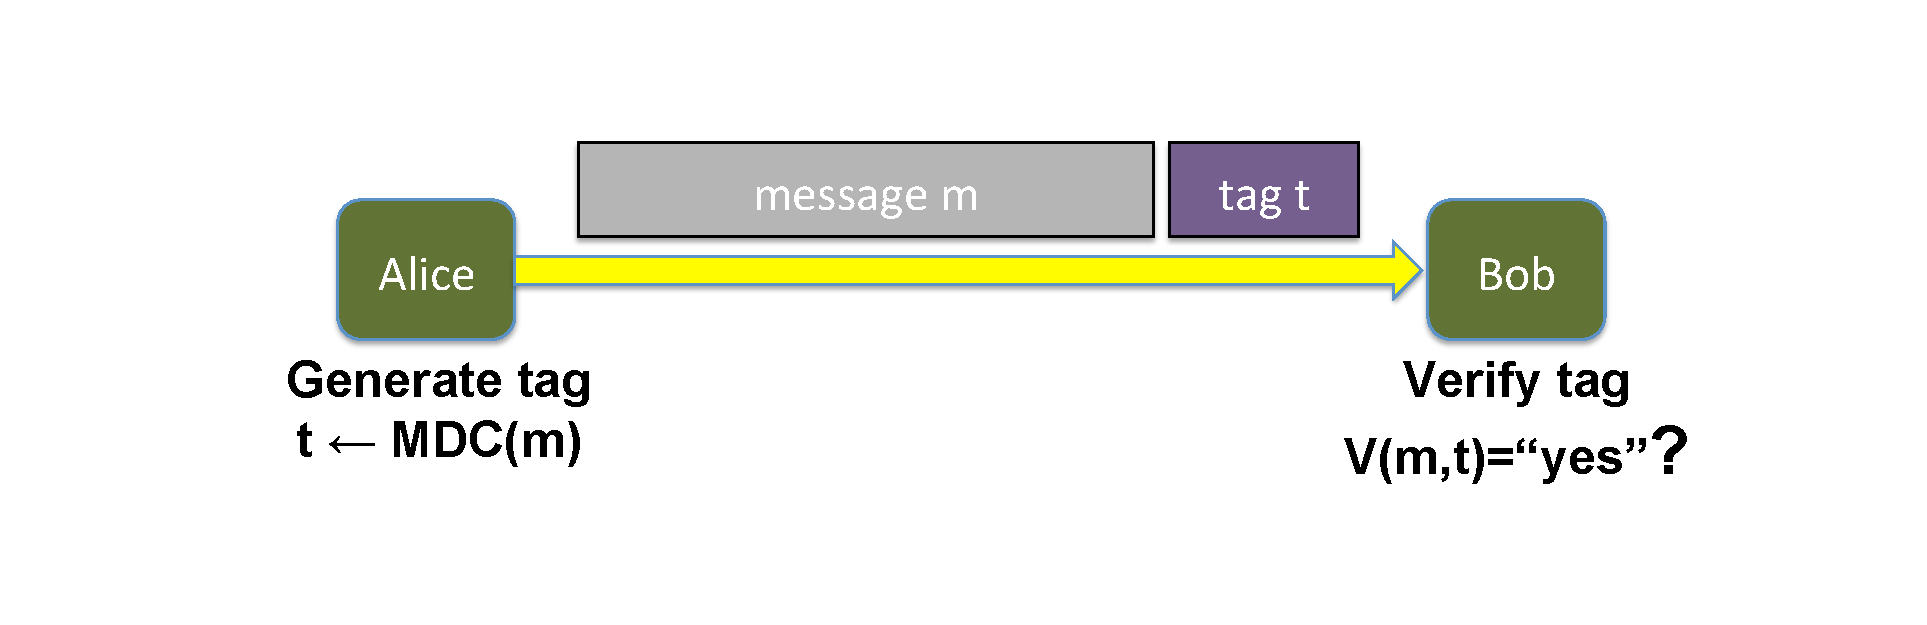
\includegraphics[scale=0.4]{images/integrity2.pdf}
    \end{tabular}
  \end{center}

  \begin{block}{MACs}
    \begin{itemize}
    \item are not publicly verifiable (and so not transferable)

      \envert{No one else, except Bob, can verify $t$.}

    \item do not provide non-repudiation

      \envert{$t$ is not bound to Alice's identity only. Alice could later claim she didn't compute $t$ herself. It could very well have been Bob since he also knows the key $k$. }
    \end{itemize}
  \end{block}

\end{frame}
  
\begin{frame}
  \frametitle{Advantages of digital signatures over MACs}

  \begin{center}
    \begin{tabular}{l}
      \includegraphics[scale=0.4]{images/integrity1.png}
    \end{tabular}
  \end{center}


  \begin{block}{Digital signatures}
    \begin{itemize}
    \item are \enbleu{publicly verifiable} - anyone can verify a signature tag $t$ (also referred to as $s$)
    \item are \enbleu{tansferable} - due to public verifiability 
    \item provide \enbleu{non-repudiation} - if Alice signs a document with $sk$, she cannot deny it later\\
        \envert{Alice is responsible for keeping her secret key $sk$ secret.}
    \end{itemize}
  \end{block}
  
\end{frame}

\begin{frame}
  \frametitle{Security}

  A good digital signature schemes should satisfy existential unforgeability.

  \begin{block}{Existential unforgeability}
    \begin{itemize}
    \item Given $(m_1, S(sk, m_1))$, \dots, $(m_n, S(sk, m_n))$ (where $m_1$, \dots, $m_n$ chosen by the adversary)
    \item It should be hard to compute a valid pair \enrouge{$(m^*, s^*)$} such that $V(pk,m^*,s^*)=1$ without knowing $sk$ for any $m^*\not\in\{m_1, \dots, m_n\} $
    \end{itemize}
  \end{block}

\end{frame}

\begin{frame}
  \frametitle{Textbook RSA signatures}

    \begin{itemize}
  \item $G_{RSA}() = (pk, sk)$ \hfill where $pk=(N, e)$ and $sk=(N,d)$

    \hfill and $N = p\cdot q$ with $p, q$ random primes

    \hfill and $e, d \in \mathbb Z$ st. $e\cdot d \equiv 1\ (\mathsf{mod}\ \phi(N))$
    \smallskip{}
    \pause

  \item $\Mcal = \mathcal{S} = \mathbb Z_N$
   \smallskip{}
    \pause

  \item Signing: $S_{RSA}(sk, x) = (x, x^d\ (\mathsf{mod}\ N))$ \hfill where $sk=(N,d)$
    \smallskip{}
    \pause

  \item Verifying: $V_{RSA}(pk, m, x) = \left\{
    \begin{array}[c]{ll}
      1 & \text{if } m = x^e\ (\mathsf{mod}\ N) \\
      0 & \text{otherwise}
    \end{array}
    \right.$
    
    where $pk=(N,e)$ 
    \smallskip{}
    \pause

  \item st $\forall (pk, sk) \in G_{RSA}()$, $\forall m \in \Mcal$, $V_{RSA}(pk, m, S_{RSA}(sk, m)) = 1$
    \pause

    \underline{Proof:} exactly as proof of consistency of RSA encryption/decryption
  \end{itemize}
\end{frame}

\begin{frame}
  \frametitle{Problems with ``textbook RSA signatures''}

  \begin{block}{Textbook RSA signatures are not secure}
    The ``textbook RSA signature'' scheme \enrouge{does not provide existential unforgeability}
  \end{block}

  \begin{itemize}
  \item Suppose Eve has two valid signatures $s_1 = m_1^d\ (\mathsf{mod}\ N)$ and $s_2 = m_2^d\ (\mathsf{mod}\ N)$ from Bob, on messages $m_1$ and $m_2$.
  \item Then Eve can exploit the homomorphic properties of RSA and produce a new signature 
    \pause
    \[
    s^* = s_1\cdot s_2\ (\mathsf{mod}\ N)=  m_1^d \cdot m_2^d\ (\mathsf{mod}\ N) = (m_1\cdot m_2)^d\ (\mathsf{mod}\ N)
    \]
    which is a valid signature from Bob on message $m_1 \cdot m_2$.
  \end{itemize}

\end{frame}

\begin{frame}
  \frametitle{How to use RSA for signatures}

  \begin{block}{Solution}
    Before computing the RSA function, apply a hash function \enrouge{H}. 
  \end{block}

  \begin{itemize}
  \item Signing: $S_{RSA}(sk, m) = \enrouge{H(}m\enrouge{)}^d\ (\mathsf{mod}\ N)$
    \smallskip{} \pause

  \item Verifying: $V_{RSA}(pk, m, s) = \left\{
      \begin{array}[c]{ll}
        1 & \text{if } \enrouge{H(}m\enrouge{)} = s^e\ (\mathsf{mod}\ N) \\
        0 & \text{otherwise}
      \end{array}
    \right.$
  \end{itemize}


\end{frame}

\coverpartname{Secure communications}
\covertopicname{Public Key Infrastructure}

\begin{frame}
  \maketitle
\end{frame}

\begin{frame}
  \frametitle{Public keys}

  \begin{figure}[c]
    \centering
    \includegraphics[scale=0.2]{images/asyouwish1.pdf}
    \caption{How does Alice trust that $\mathsf{pk}_{\mathsf{amazon}}$ is Amazon's public key?}
  \end{figure}
  \bigskip

  \begin{block}{}
    Public-key encryption schemes are secure only if the authenticity of the public key is assured
  \end{block}
\end{frame}

\begin{frame}{Distribution of public keys}
  \begin{enumerate}
  \item \enbleu{Public announcements -} participants broadcast their public key\pause

    \enrouge{\Large{\frownie}\ \normalsize does not defend against fake certificates}
    \medskip{}

  \item \enbleu{Publicly available directories -} participants publish their public key on public directories\pause

    \enrouge{\Large{\frownie}\ \normalsize does not defend against fake certificates}
    \medskip{}

  \item \enbleu{Public-key authority -} participants contact the authority for each public key it needs \pause

    \enrouge{\Large{\frownie}\ \normalsize bottleneck in the system}
    \medskip{}

  \item \enbleu{public-key certificates -} CAs issue certificates to participants on their public key \pause

    \envert{\Large{\smiley}\ \normalsize as reliable as public-key authority but avoiding the bottleneck}
    \medskip{}

  \end{enumerate}
\end{frame}

\begin{frame}{Critical step: Certificate validation}
\vspace{-0.6cm}

  \begin{columns}[t]
\hspace{-1.0cm}
\begin{column}{0.68\textwidth}
	\begin{itemize}
		\item \textbf{The crux of TLS security}: Server authenticates itself to client
		\item \textbf{What is a certificate?}
		      \begin{itemize}
			      \item A public key + signature on that key and
			      \item associated information (domain name, organization, etc.)
			       			\begin{itemize}
				            \item \enrouge{Encoded in an insanely asinine byte format}
			            \end{itemize}

			      \item Essentially says: ``I am google.com, and my public key is [key]''
		      \end{itemize}\pause
		\item \textbf{Certificate validation process}:
		      \begin{enumerate}
			      \item Browser receives certificate from server
			      \item Verifies the certificate's signature
			      \item If signature is valid \rightarrow{} certificate and public key are trusted
			      \item Browser proceeds with connection
		      \end{enumerate}
	\end{itemize}
\end{column}
\begin{column}{0.30\textwidth}
  \vspace{-1.5cm}
  \visible<1->{
    \begin{figure}[c]
    \centering
    \includegraphics[scale=0.2]{images/X509certificates.pdf}
    \caption{\scriptsize Image from Cryptography and Network Security - Principles and Practice - William Stallings}
  \end{figure}
  }
\end{column}  
\end{columns}
\end{frame}


\begin{frame}{Certificate Authorities: The trust foundation}
	\begin{itemize}
		\item \textbf{Problem}: \enrouge{Wait!} How does the browser know which public key to use for verification? \pause
		\item \textbf{Solution}: Certificate Authorities (CAs)
		      \begin{itemize}
			      \item Public keys hardcoded in your browser/OS.
			      \item Trusted organizations that issue certificates.
			      \item Act as trusted third parties. \pause
		      \end{itemize}
		\item \textbf{CA's role}:
		      \begin{itemize}
			      \item Verify that public keys belong to claimed entities.
			      \item Sign certificates with their private keys.
			      \item Protect their private keys from compromise.\pause
		      \end{itemize}
		\item \textbf{Without CAs}: No way to distinguish legitimate servers from MITM attackers!
	\end{itemize}
\end{frame}

\begin{frame}{Traditional CA validation nightmare}{Pre 2015, before Snowden}
	\begin{itemize}
		\item \textbf{Getting a certificate before 2015}:
		      \begin{itemize}
			      \item Contact a Certificate Authority (Verisign, Thawte, etc.).
			      \item Pay \$50-300+ per certificate per year.
			            \begin{itemize}
				            \item \enrouge{Completely arbitrary extortionate amounts.}
			            \end{itemize}
			      \item Manual validation process takes days/weeks.\pause
		      \end{itemize}
		\item \textbf{Domain Validation (DV) process}:
		      \begin{enumerate}
			      \item Submit CSR (Certificate Signing Request).
			      \item CA sends email to \texttt{admin@domain.com}.
			      \item Click verification link in email.
			      \item Wait for manual review and approval.
			      \item Download and install certificate.\pause
		      \end{enumerate}
		\item \textbf{Extended Validation (EV) certificates}:
		      \begin{itemize}
			      \item Even more expensive (\$150-1000+/year).
			      \item Weeks of back-and-forth communication.
		      \end{itemize}
	\end{itemize}
  \begin{textblock*}{5cm}(11cm,1cm)
    \begin{figure}
\includegraphics[width=4cm]{images/snowden.png}
\caption{{\scriptsize Edward Snowden in 2013, Wikipedia}}
  \end{figure}
\end{textblock*}
\end{frame}

\begin{frame}{Let's Encrypt: revolution in TLS certificates (2015)}
	\begin{itemize}
		\item \textbf{Game-changing}:
		      \begin{itemize}
			      \item \textbf{Free} certificates for everyone.
			      \item \textbf{Automated} issuance and renewal.
			      \item \textbf{90-day} certificate lifetime (encourages automation).
			      \item Open source, non-profit initiative.\pause
		      \end{itemize}
		\item \textbf{ACME protocol} (Automated Certificate Management Environment):
		      \begin{itemize}
			      \item Domain validation via HTTP or DNS challenges.
			      \item Prove control of domain programmatically.
			      \item Certificate issued in seconds, not days.
			      \item Automatic renewal before expiration.\pause
		      \end{itemize}
		\item \textbf{Impact on the web}:
		      \begin{itemize}
			      \item HTTPS adoption jumped from 40\% to 90\%+ of web traffic.
			      \item Eliminated cost barrier for small websites.
			      \item Made ``HTTPS everywhere'' a reality.\pause
		      \end{itemize}
		\item \textbf{Philosophy}: Encryption should be the default, not a luxury.
	\end{itemize}
\end{frame}

\begin{frame}{Let's Encrypt: active certificates}
	\bigimagewithcaption{letsencrypt-certs.png}{Source: Let's Encrypt}
\end{frame}

\begin{frame}{Let's Encrypt: certificates issued}
	\bigimagewithcaption{letsencrypt-issuance.png}{Source: Let's Encrypt}
\end{frame}

\begin{frame}{Percentage of HTTPS traffic in Firefox}
	\bigimagewithcaption{letsencrypt-https.png}{Source: Let's Encrypt}
\end{frame}

\begin{frame}{Certificate chains in practice}
	\begin{itemize}
		\item \textbf{Real-world example}: Connecting to \texttt{www.google.com}
		\item \textbf{Certificate chain structure}:
		      \begin{itemize}
			      \item \textbf{Certificate 0}: \texttt{www.google.com}'s certificate.
			      \item \textbf{Certificate 1}: Intermediate CA (Google Trust Services).
			      \item \textbf{Certificate 2}: Root CA (GlobalSign).
		      \end{itemize}
		\item \textbf{Verification process}:
		      \begin{enumerate}
			      \item Check Google's signature on Certificate 0.\pause
			      \item Check GlobalSign's signature on Certificate 1.\pause
			      \item Trust GlobalSign's root certificate (pre-installed).\pause
		      \end{enumerate}
		\item \textbf{Chain of trust}: Each certificate vouches for the next.
	\end{itemize}
\end{frame}

\begin{frame}{Exploring certificates with OpenSSL}
	\begin{itemize}
		\item \textbf{Connect and view certificate}:
		      \begin{itemize}
			      \item \texttt{openssl s\_client -connect www.google.com:443}
			      \item Shows certificate chain and raw certificate data \pause
		      \end{itemize}
		\item \textbf{Parse certificate details}:
		      \begin{itemize}
			      \item \texttt{openssl x509 -text -noout}
			      \item Reveals subject, issuer, validity dates, algorithms\pause
		      \end{itemize}
		\item \textbf{Certificate markers}:
		      \begin{itemize}
			      \item \texttt{s:} = subject (who the certificate is for)
			      \item \texttt{i:} = issuer (who signed the certificate)\pause
		      \end{itemize}
		\item Try this at home! Great way to understand the certificate ecosystem.\\ \ \\
    
    \texttt{openssl s\_client -connect www.google.com:443 -servername www.google.com | openssl x509 -text -noout}
	\end{itemize}
\end{frame}

\iffalse
\begin{frame}
  \frametitle{Public key certificates}
  \vspace{-0.65cm}

  \begin{figure}[c]
    \centering
    \includegraphics[scale=0.3]{images/PublicKeyCertificate.pdf}
    \caption{\scriptsize image from Cryptography and Network Security - Principles and Practice - William Stallings }
  \end{figure}
  \vspace{-0.25cm}


  \begin{block}{A certificate consists mainly of }
    \begin{itemize}
    \item a \enbleu{public key}
    \item a \enbleu{subject} identifying the owner of the key
    \item a \enbleu{signature} by the CA on the key and the subject binding them together

      \enrouge{the CA is trusted}
    \end{itemize}
  \end{block}

\end{frame}

\begin{frame}
  \frametitle{X.509 certificates}

  \begin{figure}[c]
    \centering
    \includegraphics[scale=0.3]{images/X509certificates.pdf}
    \caption{\scriptsize image from Cryptography and Network Security - Principles and Practice - William Stallings}
  \end{figure}

  \begin{itemize}
  \item X.509 defines a framework for the provision of authentication services
  \item Used by many applications such as TLS
  \end{itemize}
\end{frame}
\fi

\begin{frame}
  \frametitle{Public key certificates}
  \begin{figure}[c]
    \centering
    \includegraphics[scale=0.2]{images/asyouwish2.pdf}
    \caption{Alice can now verify Amazon's certificate}
  \end{figure}

\end{frame}

\begin{frame}
  \frametitle{Using public key certificates to secure the Internet}
  \vspace{-0.45cm}
  \begin{center}
    \includegraphics[scale=0.45]{images/AmazonWebsite.pdf}
  \end{center}


  \begin{block}{A very important implicit assumption}
    The browser is trusted to be ``secure''
  \end{block}
\end{frame}

\begin{frame}
  \frametitle{Amazon's certificate}
    \vspace{-0.45cm}
  \begin{center}
    \includegraphics[scale=0.3]{images/AmazonCertificate.pdf}
  \end{center}

\end{frame}

\begin{frame}{Browser root certificates}
      \vspace{-0.45cm}
  \begin{center}
    \includegraphics[scale=0.3]{images/RootCertificates.pdf}
  \end{center}

\end{frame}

\iffalse
\begin{frame}{Chain of trust}
    \vspace{-0.45cm}
  \begin{figure}[c]
    \centering
    \includegraphics[scale=0.5]{images/Hierarchy.pdf}
    \caption{\scriptsize X.509 Hierarchy - image from Cryptography and Network Security - Principles and Practice - William Stallings}
  \end{figure}

  \begin{block}{}
    \begin{itemize}
    \item Having a single CA sign all certificates is not practical
    \item Instead a root CA signs certificates for level 1 CAs, level
      1 CAs sign certificates for level 2 CAs, \emph{etc}
    \end{itemize}
  \end{block}

\end{frame}


\begin{frame}{Self-signed certificates}

  \begin{center}
    \includegraphics[scale=0.4]{images/selfsignedcertificate.pdf}
  \end{center}

\end{frame}

\begin{frame}
      \vspace{-0.45cm}
  \frametitle{The Lenovo Superfish scandal (February 2015)}
  \begin{center}
    \includegraphics[scale=0.65]{images/LenovoSuperfish.pdf}
  \end{center}
\end{frame}

\begin{frame}
  \frametitle{And another scandal (September 2016)}

  \begin{center}
    \includegraphics[scale=0.85]{images/WoSign.pdf}
  \end{center}

\end{frame}
\fi

\begin{frame}{Revocation}
    \vspace{-0.45cm}
    A certificate needs to be revoked if the corresponding private key has been compromised.\bigskip
    \begin{itemize}
    \item   Partly solved by short-lived certificates (e.g., Let's Encrypt certificates are valid for 90 days only).\bigskip\pause
      
    \item   Certificate Revocation Lists (CRLs) are the solution adopted in X.509.\bigskip\pause
      
    \item Online Certificate Status Protocol (OCSP) stapling is the modern solution to this problem \envert{ -- basically two certificates, one for the content, one for the validity}. \pause
    \end{itemize}

  \end{frame}

\end{document}
